% ###################################################################################################
% Chapter 8 - Survival and Health Mechanics
% ###################################################################################################
\chapter{Survival Mechanics}

\begin{figure}[h]
    \centering
    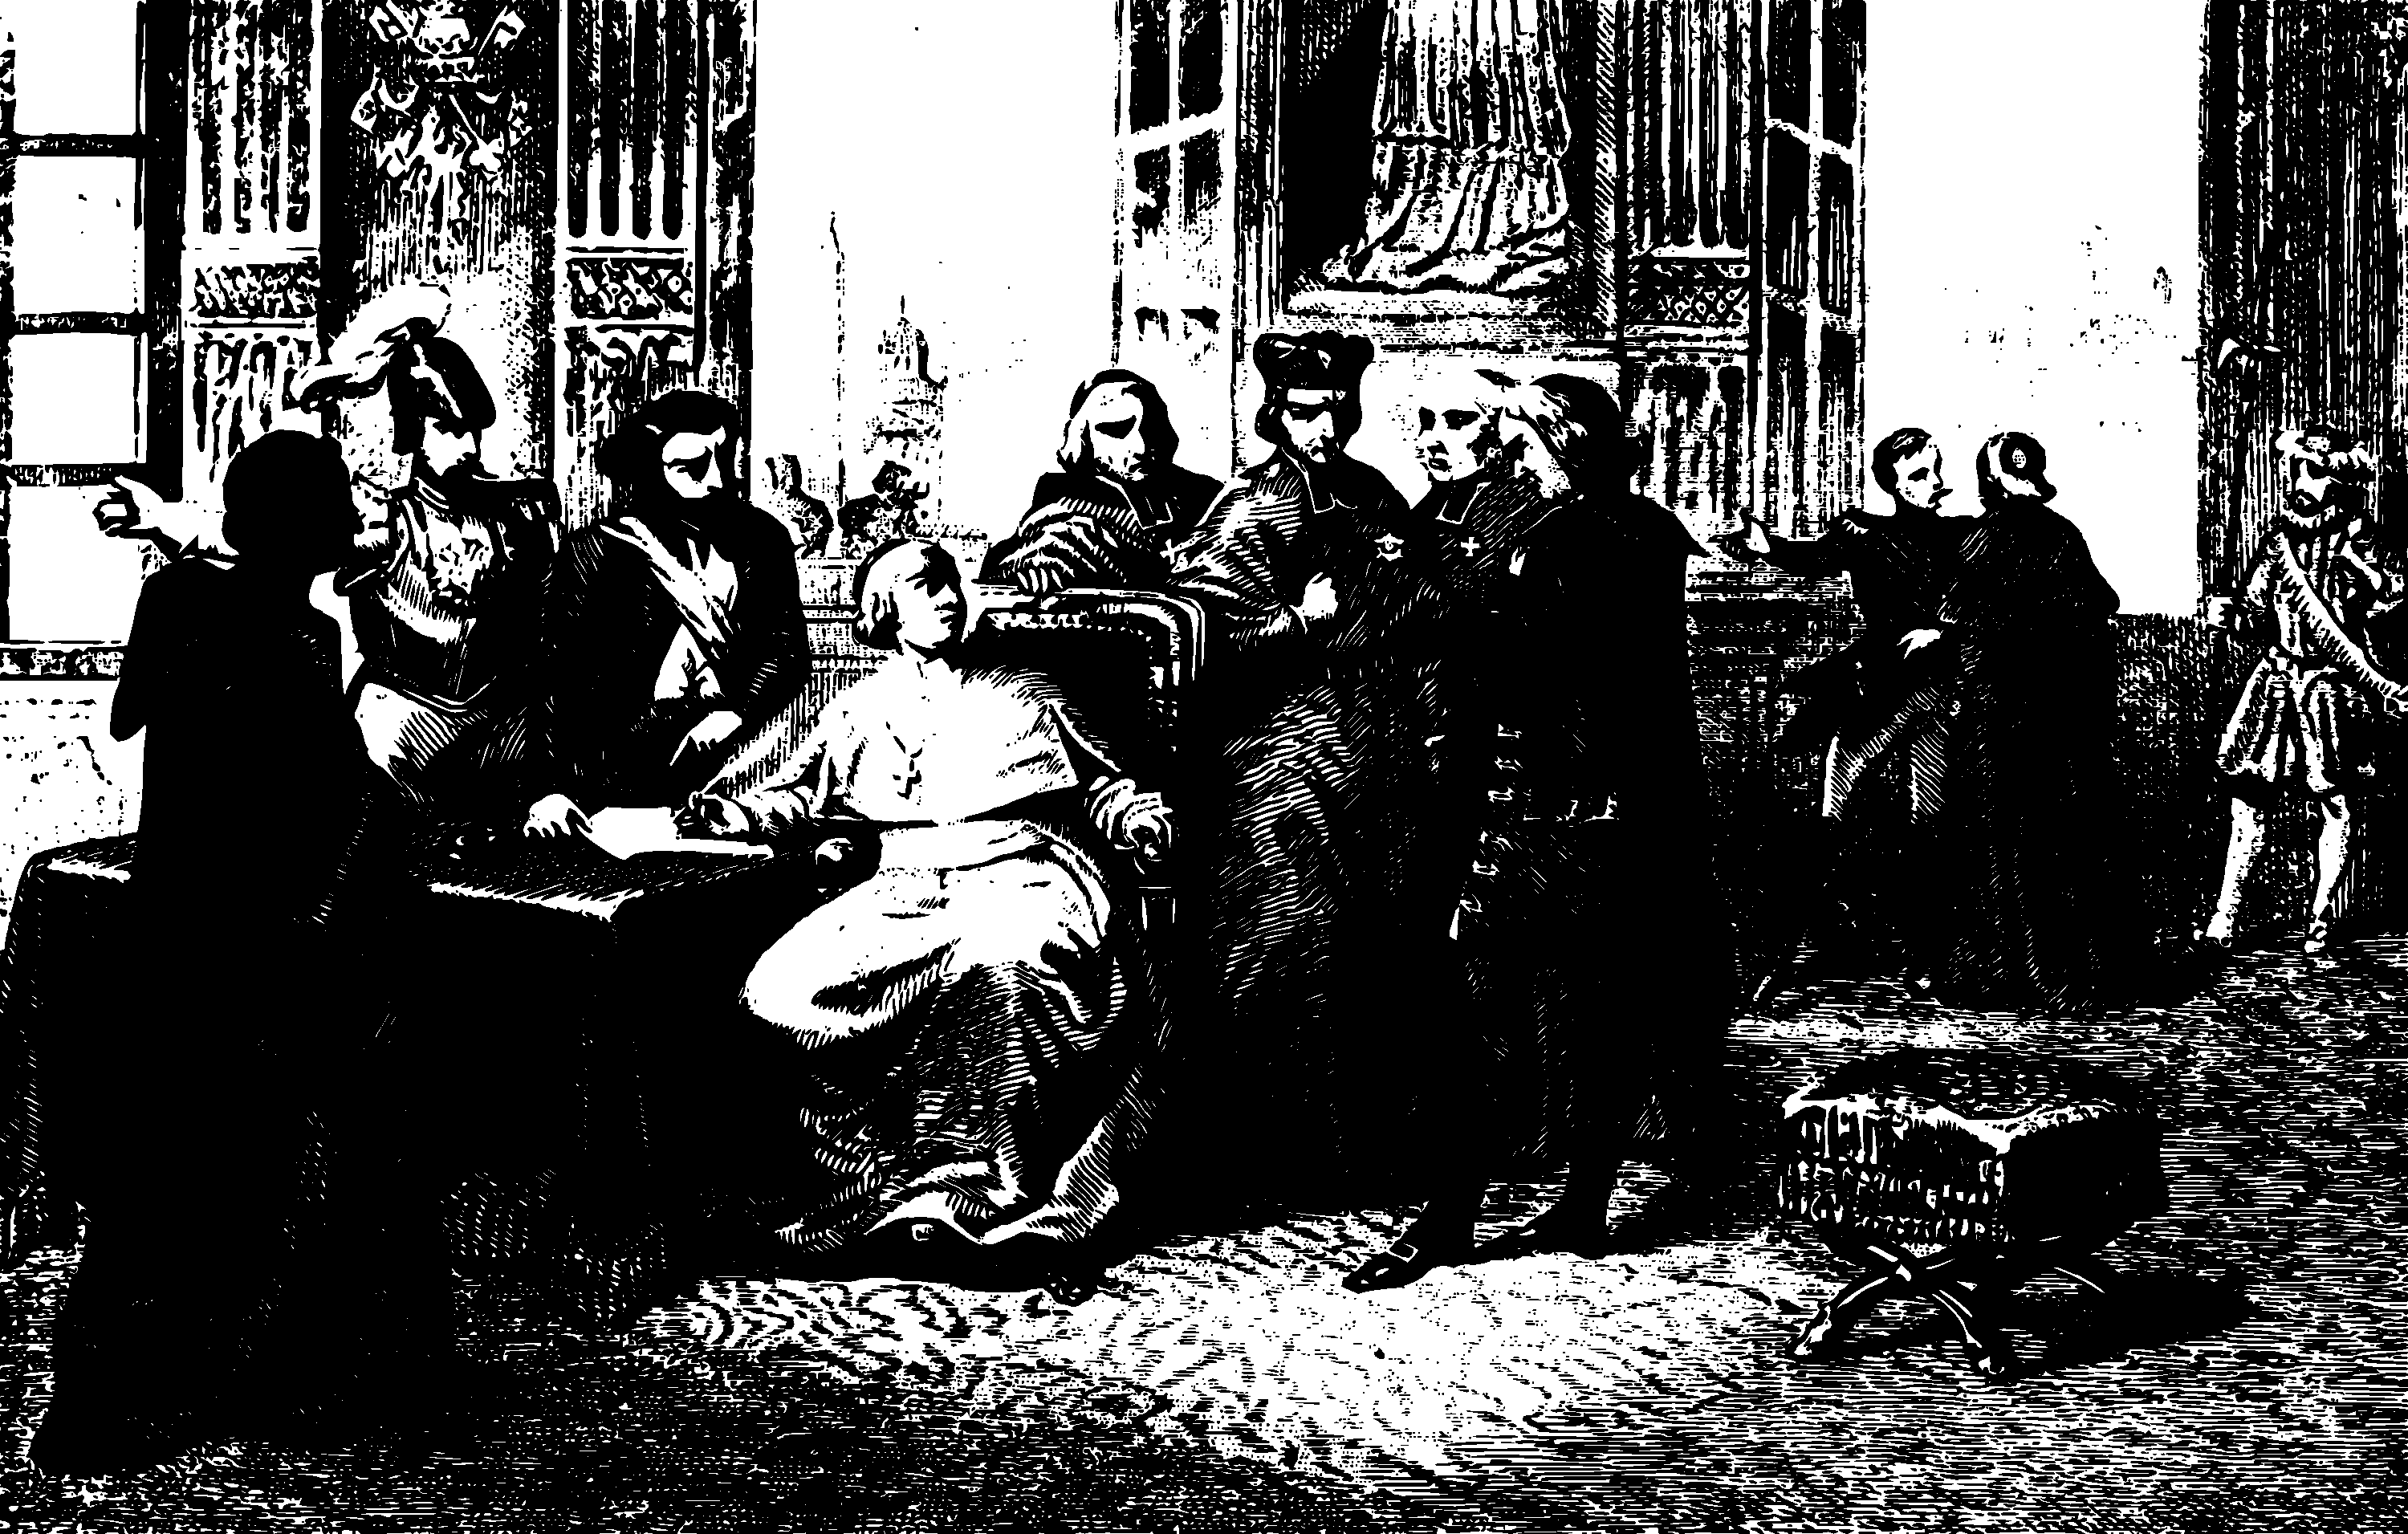
\includegraphics[width=\textwidth]{./images/survival01.pdf}
    % \caption{Inline Example Image}
\end{figure}

Survival in Eidos revolves around the balance between risk and resilience. When characters face environmental challenges, hunger, thirst, or wounds, their effectiveness declines—but these conditions also provide narrative depth, giving the GM and players opportunities to explore moments of hardship and triumph.

\section{Food and Water Requirements}

Survival depends on the characters managing hunger and thirst. These conditions are tracked narratively rather than with numbers. Going without food or water introduces nerfs to skill tests, symbolizing fatigue, confusion, or irritability.

\textbf{Hungry:} -1 to mental rolls (distraction from hunger).

\textbf{Thirsty:} -1 to physical rolls (muscle weakness or slowed reflexes).

After one full day without food or water, these penalties increase to -2. At this stage, the character may exhibit behavioral shifts such as irritability, sluggishness, or hallucinations—elements that drive the narrative. Players must seek sustenance within the story through scavenging, hunting, or trading. Eating and drinking restore the character to normal functionality.

\section{Shelter and Environmental Hazards}

Exposure to extreme weather or dangerous environments gradually wears down a character through Fatigue Points:

\begin{itemize}
    \item \textbf{1-2 Points:} Minor exhaustion (no effect).
    \item \textbf{3-4 Points:} -1 to all physical rolls.
    \item \textbf{5+ Points:} Risk of unconsciousness (character must roll 2d20 against a target of 15).
\end{itemize}

To recover, the player must find shelter (a warm camp, dry cave, or safe house). GMs can use these rest moments to introduce story hooks, like meeting NPCs or making discoveries. Shelter also restores 1 Fatigue Point per hour of uninterrupted rest.

\section{Scavenging and Resource Management}

In Eidos, scavenging is an exploratory mechanic driven by narrative. Instead of predefined loot tables, the GM describes environments and players declare their intentions (e.g., “I search the abandoned warehouse for water containers”). Each scavenging action requires a 2d20 roll:

\begin{itemize}
    \item \textbf{Success:} The player finds useful supplies (food, water, first aid).
    \item \textbf{Partial success:} The item is damaged or in limited supply.
    \item \textbf{Failure:} The player finds nothing or risks a complication (like setting off an alarm or encountering a hostile creature).
\end{itemize}

Resources like food, water, or bandages aren’t counted individually but treated as narrative elements. For example, finding a first aid kit doesn’t guarantee endless healing—it provides one meaningful use within the story.

\section{Status Effects and Debuffs}

Injuries and conditions introduce status effects that evolve with the story. These effects aren’t just penalties—they shape how characters interact with the world. Below are a few common status effects:

\begin{itemize}
    \item \textbf{Fatigued:} -1 to all rolls (can accumulate with hunger/thirst).
    \item \textbf{Infected Wound:} Must succeed in a 2d20 Survival roll every day (Difficulty 15) or the condition worsens.
    \item \textbf{Disoriented:} -2 to mental rolls (due to concussion or exhaustion).
\end{itemize}

\subsection{Resolving Status Effects}

These effects persist until addressed in the story. For example, to remove \textbf{Disorientation}, the character might need to sleep or drink water.

\section{Travel and Wilderness Exploration}

Overland travel in Eidos is measured in hours rather than hexes, prioritizing the narrative journey. A typical party traveling on foot covers approximately **20 miles per day** under normal conditions. 

\subsection{Terrain and Climate Multipliers}

The GM applies multipliers to the daily travel distance based on the terrain:
\begin{itemize}
    \item \textbf{Highways and Flat Grasslands:} $\times 1.0$ (Normal speed).
    \item \textbf{Dense Forests and Hills:} $\times 0.75$ (Reduced speed).
    \item \textbf{Swamps and High Mountains:} $\times 0.50$ (Severe impediment).
\end{itemize}

\subsection{Navigating and Getting Lost}

When traversing uncharted wilderness, the party's navigator must roll a **2d20 + MND + Survival/Navigation** check at the start of each day.
\begin{itemize}
    \item \textbf{TN 15 (Clear weather):} Success ensures the party maintains their course. Failure means they veer off course, losing 1d4 hours of travel time backtracking.
    \item \textbf{TN 20 (Stormy weather/Dense fog):} Failure results in the party becoming completely lost, wandering into uncharted (and potentially dangerous) territory.
\end{itemize}

\section{Fatigue Point Accumulation}

Fatigue represents physical exhaustion, sleep deprivation, or environmental strain. In addition to weather exposure, characters gain **Fatigue Points** under the following conditions:
\begin{itemize}
    \item \textbf{Forced March:} Traveling for more than 8 hours in a single day adds 1 Fatigue Point per hour of extra travel.
    \item \textbf{Sleep Deprivation:} Going 24 hours without an uninterrupted 8-hour sleep adds 2 Fatigue Points.
    \item \textbf{Extreme Environments:} Traveling through deserts or frozen wastes without specialized clothing adds 1 Fatigue Point every 2 hours.
\end{itemize}

\section{Scavenging Difficulty Targets}

When characters scavenge for resources (Section 3), the GM determines the success threshold using the standard 2d20 target numbers:
\begin{itemize}
    \item \textbf{TN 10 (Abundant Areas):} Looted campsites, orchards, or fresh streams.
    \item \textbf{TN 15 (Moderate Areas):} Abandoned villages, sparse forests, or rocky hills.
    \item \textbf{TN 20 (Barren Areas):} Scorched fields, ruined cities, or deep deserts.
\end{itemize}

\section{Healing and Trauma Recovery}

Physical injuries suffered from the Critical Injury tables (Chapter 7) list recovery periods (e.g., 1d4 days or weeks). Eidos provides a structured system to resolve these recovery times.

\subsection{Natural Recovery and Rest}
* **Fatigue Recovery:** A character recovers 1 Fatigue Point per hour of restful camp in a safe shelter, and recovers all Fatigue Points after a full 8-hour sleep.
* **Minor Wounds:** Scratches and bruises heal automatically after 1d4 hours of rest.

\subsection{Active Medical Treatment}
For severe wounds (days or weeks of recovery), the patient must remain resting. Another character can tend to their wounds using a **First Aid Kit** (Chapter 6) and rolling a **Medicine** check (**2d20 + MND + Medicine**):
\begin{itemize}
    \item \textbf{Success (TN 15):} The caregiver successfully treats the wound. The patient's remaining recovery time is reduced by 1 additional day (or 1 additional week for long-term trauma).
    \item \textbf{Failure:} The wound heals at the normal rate.
    \item \textbf{Critical Failure (Either die rolls a natural 1):} The wound becomes an **Infected Wound**.
\end{itemize}

\subsection{First Aid in Combat}
A character can spend their action in combat to apply first aid to a dying or heavily bleeding ally. Doing so requires a **First Aid Kit** charge and a success on a **TN 15 Medicine** check. On a success, the target is stabilized and any ongoing "Bleeding" condition is immediately resolved.

\begin{figure}[h]
    \centering
    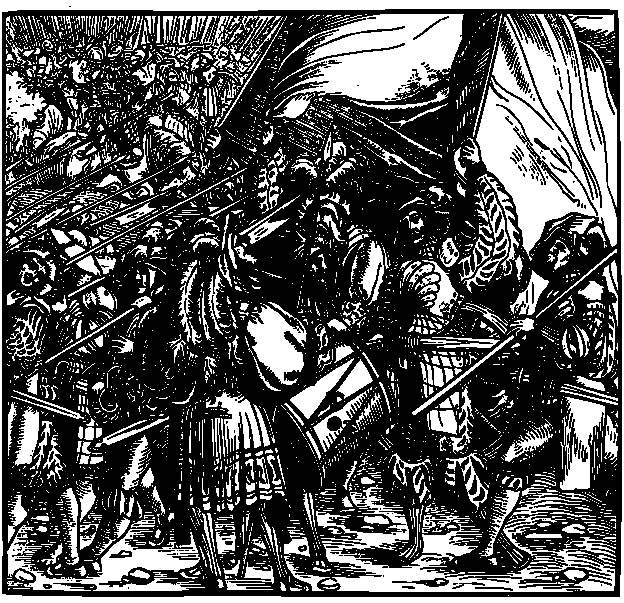
\includegraphics[width=\textwidth]{./images/survival02.pdf}
    % \caption{Inline Example Image}
\end{figure}

